\documentclass{article}
\usepackage[utf8]{inputenc}
\usepackage{amsmath,amssymb}
\usepackage{graphicx}
\usepackage[a4paper,margin=0.9cm]{geometry}
\usepackage{multicol}
\usepackage{sectsty}

\graphicspath{ {.} }

\DeclareMathOperator{\ima}{Im}
\newcommand\tab[1][0,5cm]{\hspace*{#1}}

\begin{document}
	%\allsectionsfont{\small}
	%\scriptsize
	
	\mbox{}
	\vspace{10cm}
	\begin{center}
		\textbf{\Huge{Diode}}\\
		\bigskip
		\Large{Tommaso Bertelli}\\
		\bigskip
		\Large{CO-526-B - Electronics Lab}\\
		\bigskip
		\Large{Instructor Uwe Pagel}\\
		\bigskip
		\Large{24/11/2024}\\
	\end{center}
	\pagebreak
	
	\section{Introduction - Prelab}
	\subsection{Simulation of a Differential Amplifier}
		\begin{enumerate}
			\item 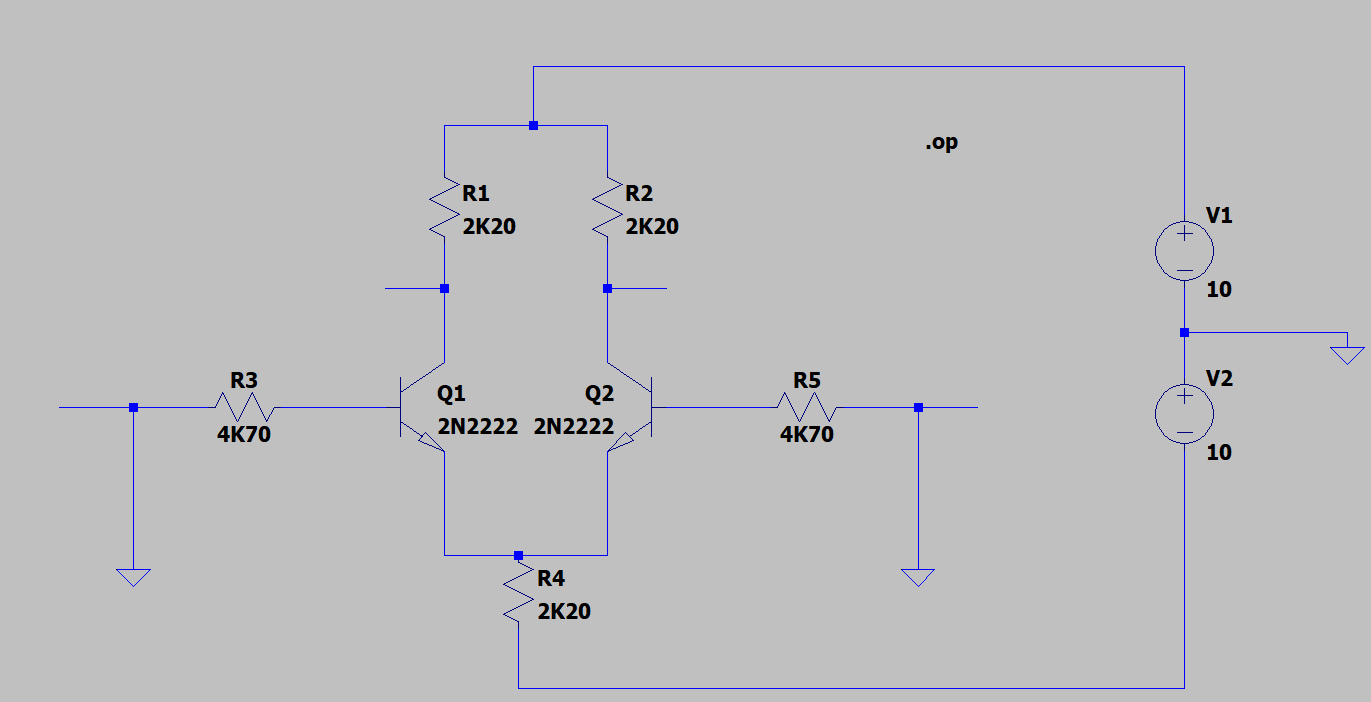
\includegraphics[scale=0.4]{circuit 1 - no input}\\\\
			\textbf{Measured voltages and currents:}\\
			\(V_{BE}\) = -47.09 - (-720.71) = 767.8mV,  \(V_C\) = 5.382V, \(I_C\) = 2.099mA, \(I_E\) = 2.109mA, \(I_{RE}\) = 4.219mA.\\\\
			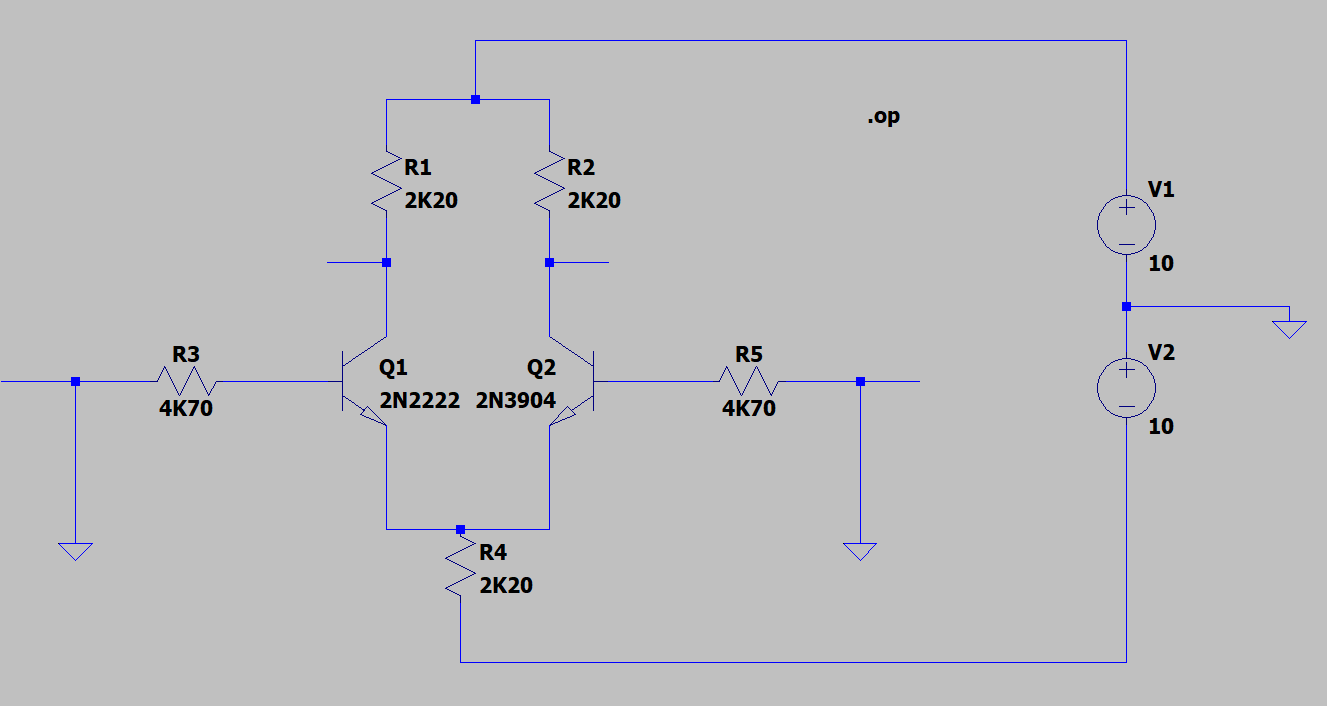
\includegraphics[scale=0.4]{circuit 1 - tr changed}\\\\
			By changing one transistor the \(V_{BE}\), \(V_C\), \(I_C\), \(I_E\) values are not symmetric anymore (ex.: \(V_C\)(Q1) = 5.911V, \(V_C\)(Q2) = 4.837V), therefore the circuit cannot work properly.
			\item \textbf{Single ended input analysis}\\\\
			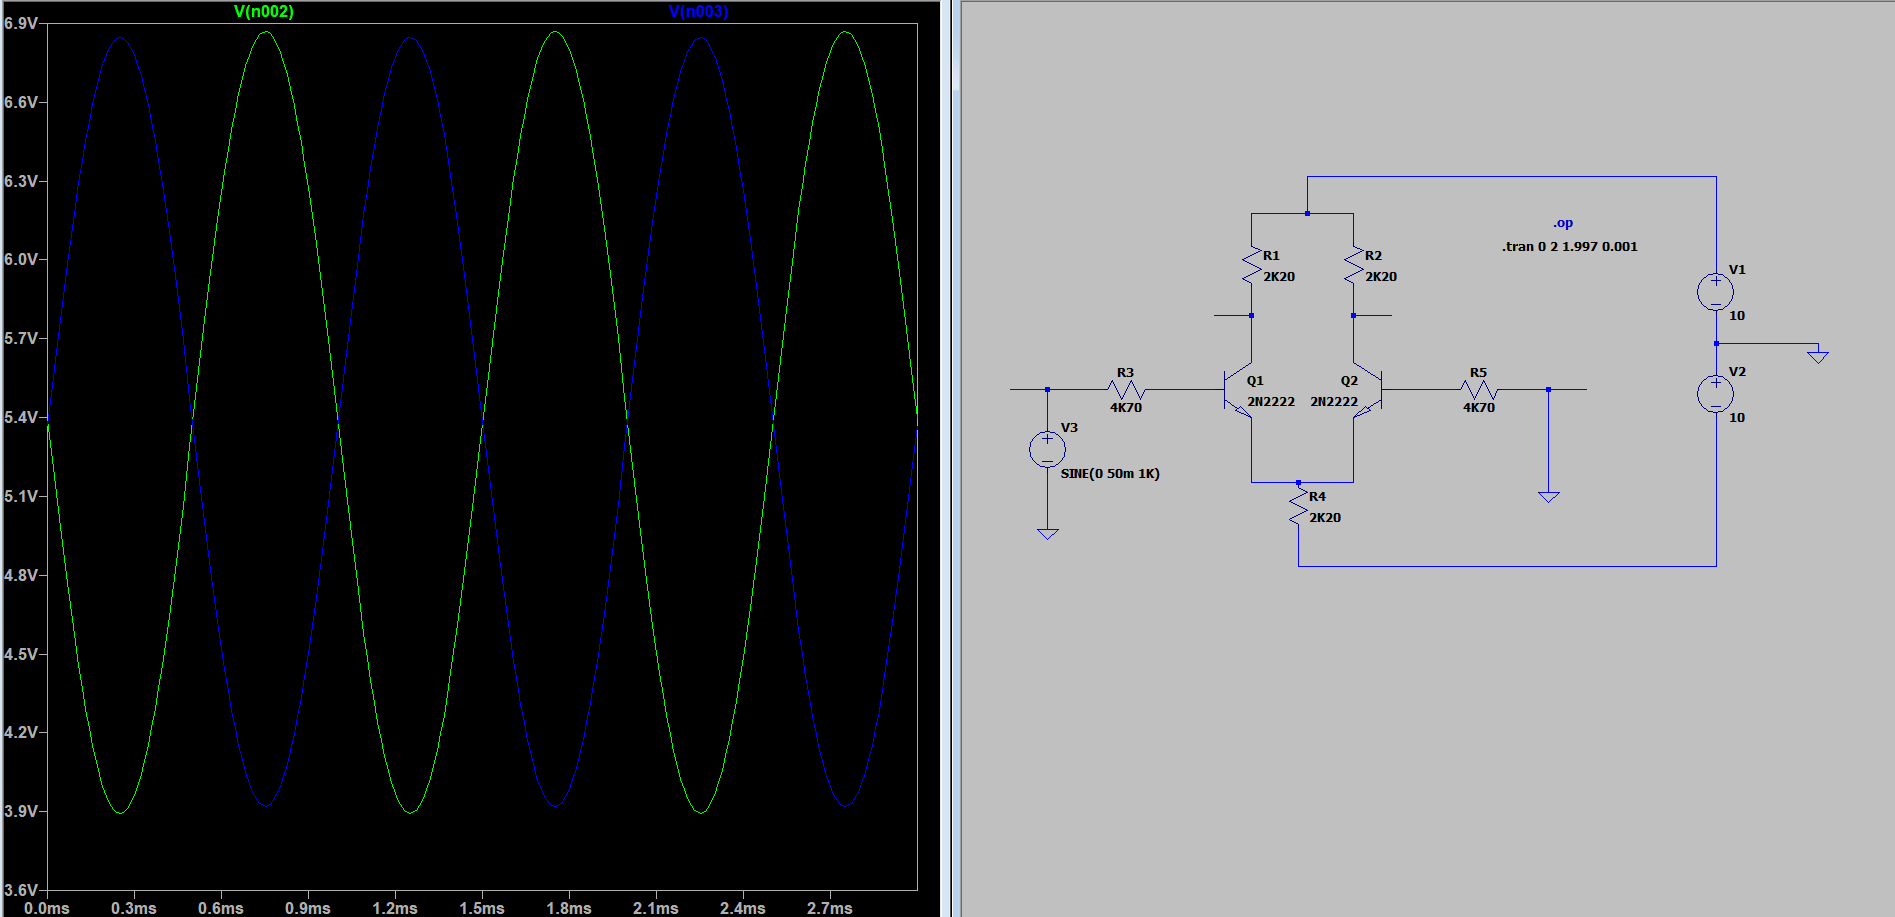
\includegraphics[scale=0.4]{circuit 2 - coll voltages}\\\\
			Green line: \(V_C\)(Q1), blue line: \(V_C\)(Q2). (peak to peak: 2.923V)\\\\\\\\\\
			To calculate \(A_{Vdiff}\) I need \(V_{od}\) and \(V_{id}\).\\\\
			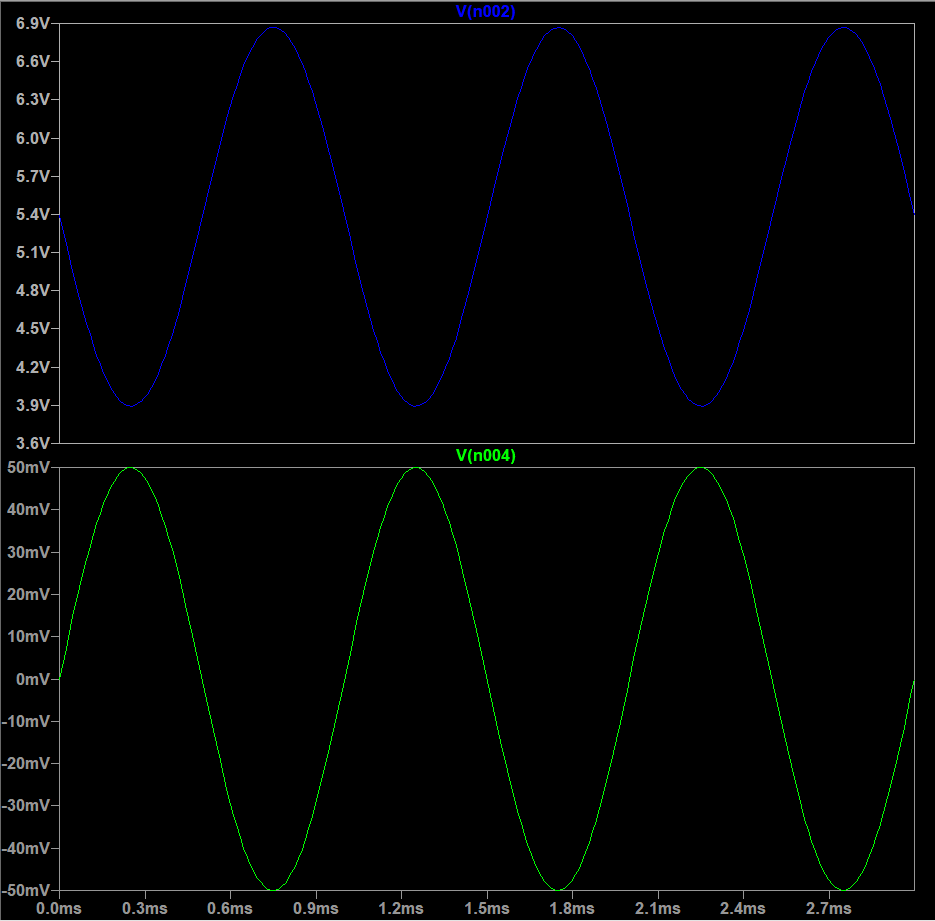
\includegraphics[scale=0.6]{circuit 2 - adiff}\\\\
			Top pane: \(V_{o1}\), bottom pane: \(V_{i1}\)\\
			\(V_{id}\) = \(V_{i1} - V_{i2}\) = 100mV peak to peak\\
			\(V_{od}\) = \(V_{o1}\) = 3V peak to peak\\
			\(A_{Vdiff} = 20log(\frac{V_{od}}{V_{id}}) \)= 29.5 dB.\\\\
			\pagebreak
			\item  \textbf{Common mode input analysis}\\\\
			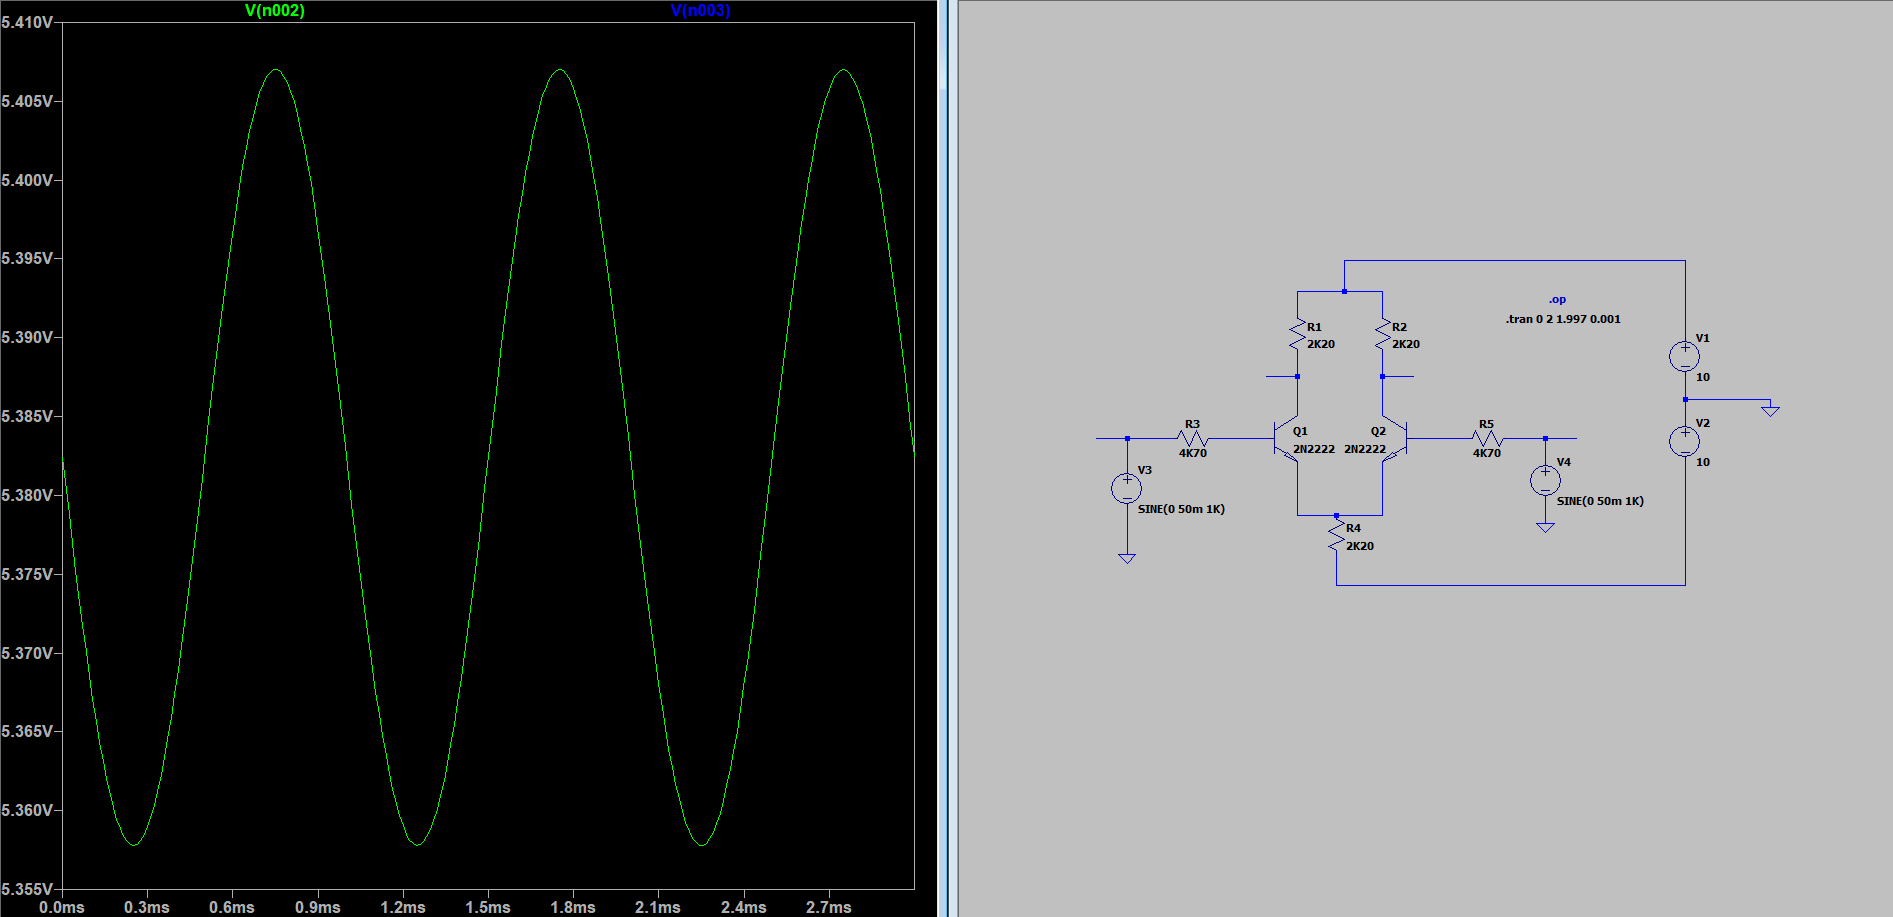
\includegraphics[scale=0.4]{circuit 3 - coll voltages}\\\\
			\(V_C\)(Q1) and \(V_C\)(Q2) are overlapping. (peak to peak: 49.17mV).\\
			To calculate \(A_{Vcm}\) I need \(V_{oc}\) and \(V_{ic}\).\\\\
			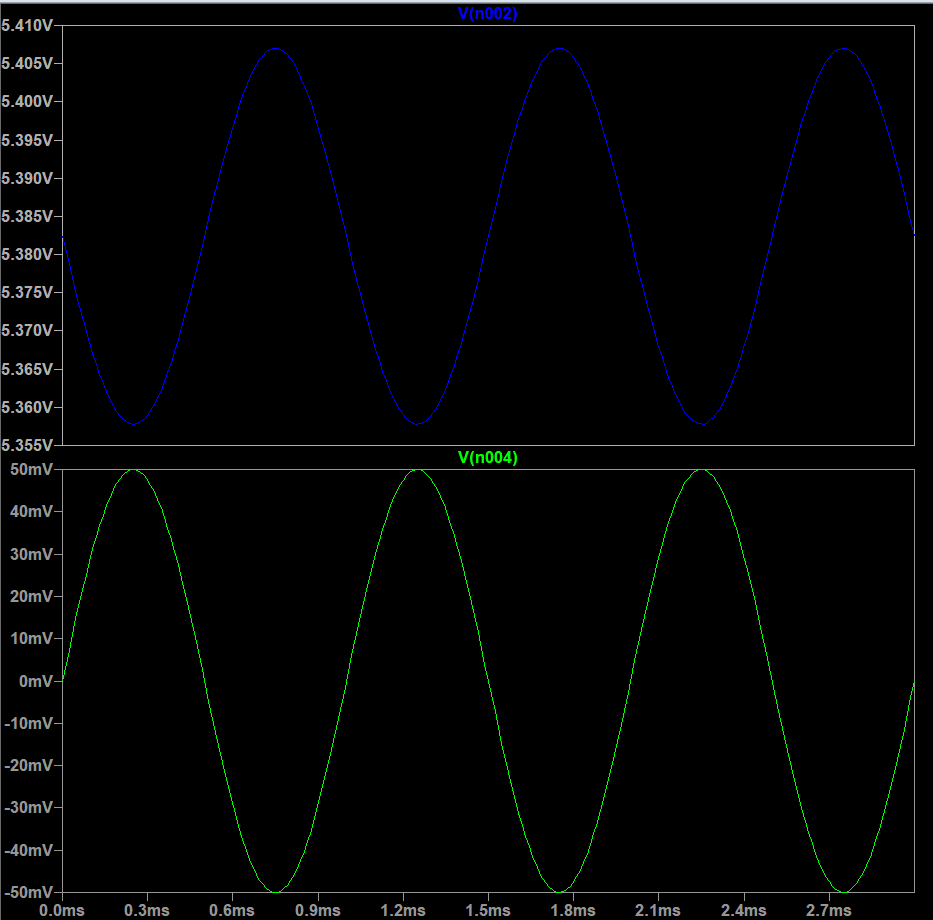
\includegraphics[scale=0.6]{circuit 2 - avcm}\\\\
			Top pane: \(V_{o1}\), bottom pane: \(V_{i1}\)\\\\
			\(V_{ic}\) = \((V_{i1} + V_{i2})/2\) = 100mV peak to peak\\
			\(V_{oc}\) = \(V_{o1}\) = 49.18mV peak to peak\\
			\(A_{Vcm} = 20log(\frac{V_{oc}}{V_{ic}}) \)= -6.16 dB.\\\\
			\item \textbf{Common mode rejection}\\\\
			\(CMRR = 20 log (\frac{A_{Vdiff}}{A_Vcm}) \)= 35.7dB.\\
			\pagebreak
			current source: 4.219 from top to bottom
			\item \textbf{Replacing R4 by equivalent current source}\\\\
			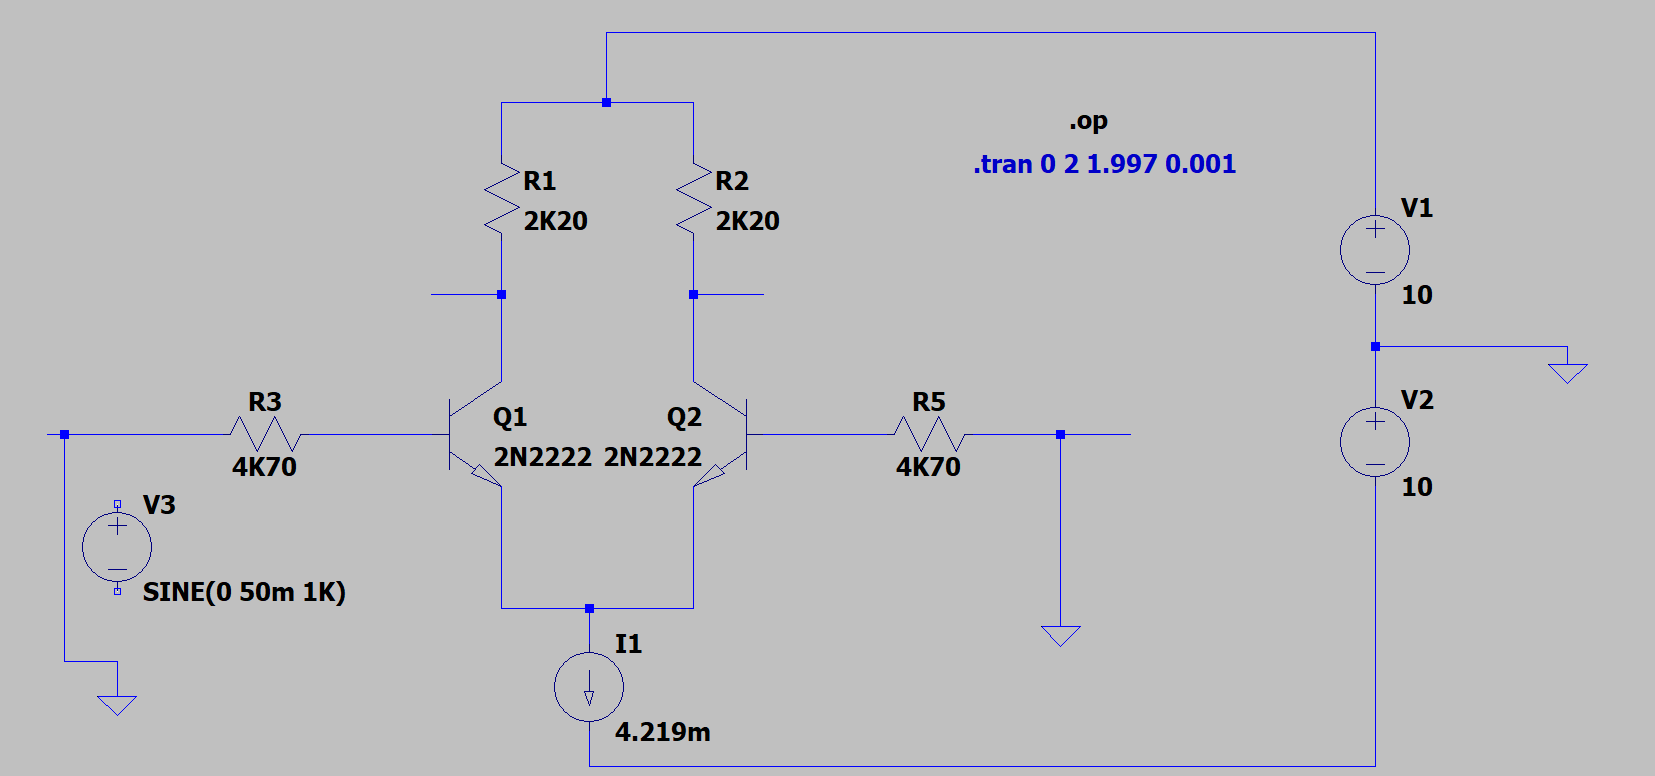
\includegraphics[scale=0.4]{circuit 5}
			\item \textbf{Analyses using the current source}
			\begin{enumerate}
				\item \textbf{DC operation point analysis}\\\\
				
				\(V_{BE}\) = -47.11 - (-720.74) = 767.85mV,  \(V_C\) = 5.381V, \(I_C\) = 2.099mA, \(I_E\) = 2.109mA, \(I_{RE}\) = 4.219mA. (current source)\\\\
				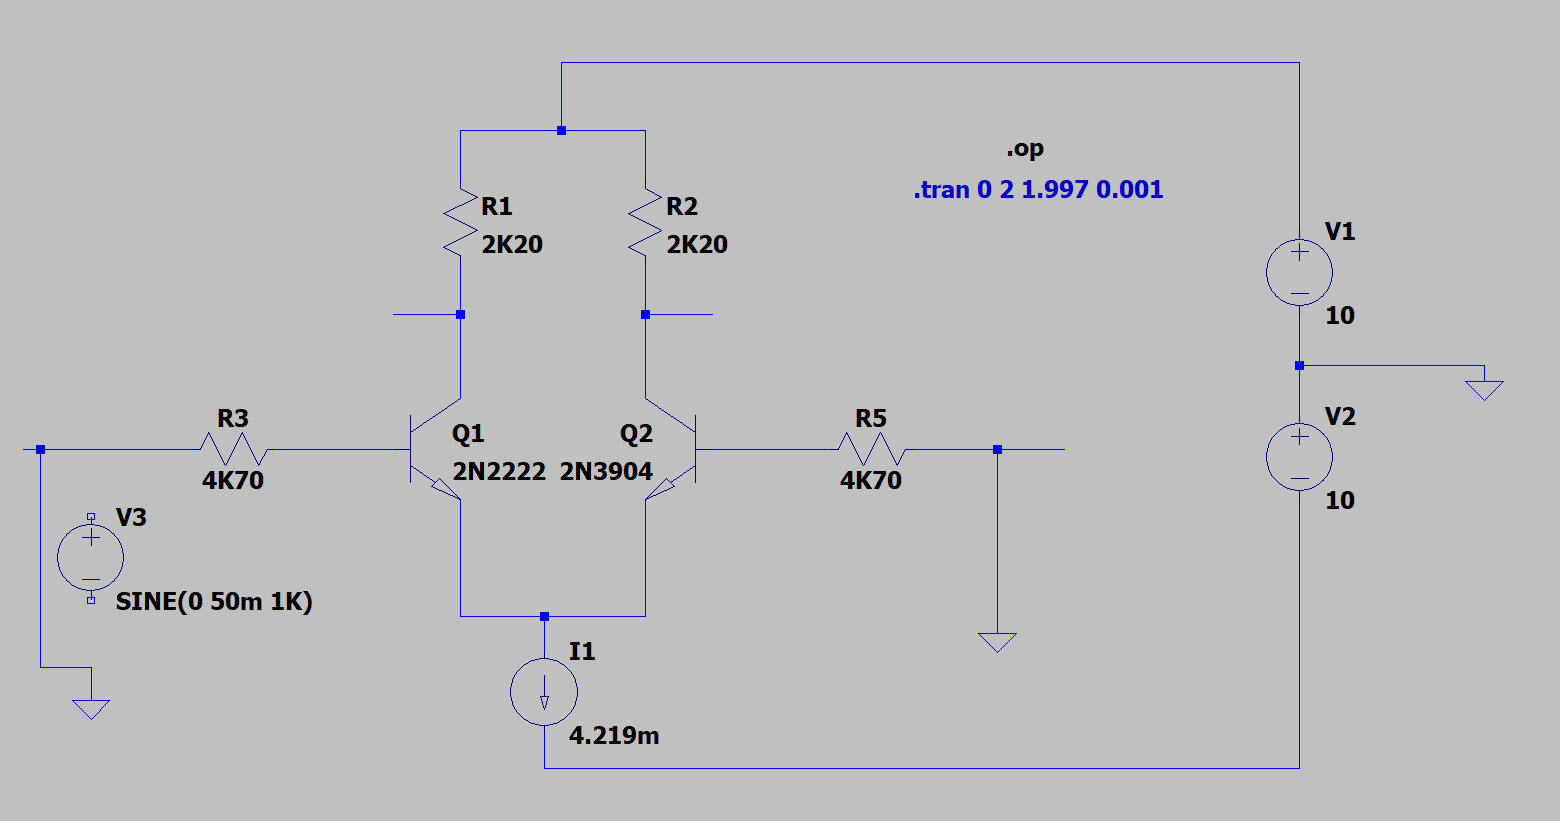
\includegraphics[scale=0.4]{circuit 5 - tr changed}\\\\
				By changing one transistor the \(V_{BE}\), \(V_C\), \(I_C\), \(I_E\) values are not symmetric anymore (ex.: \(V_C\)(Q1) = 5.913V, \(V_C\)(Q2) = 4.841V), therefore the circuit cannot work properly.\\\\
				\pagebreak
				\item \textbf{Single ended input analysis}\\\\
				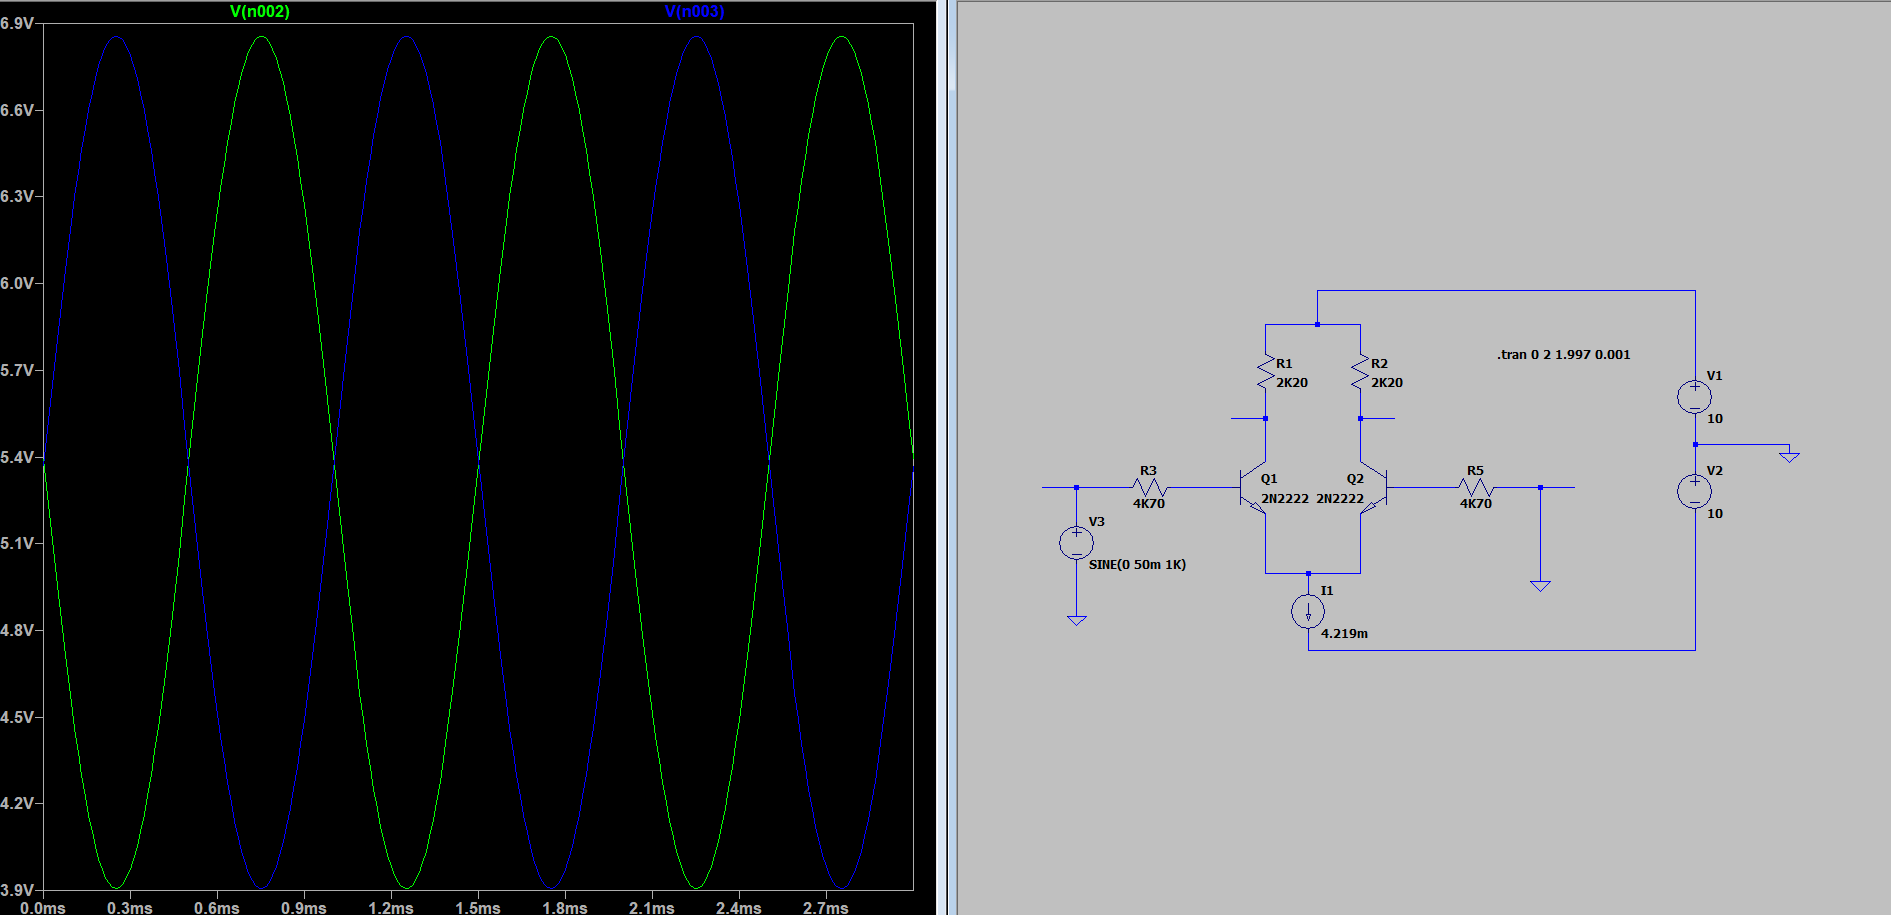
\includegraphics[scale=0.4]{circuit 6 - coll voltages}\\\\
				Green line: \(V_C\)(Q1), blue line: \(V_C\)(Q2). (peak to peak: 2.95V)\\\\
				To calculate \(A_{Vdiff}\) I need \(V_{od}\) and \(V_{id}\).\\\\
				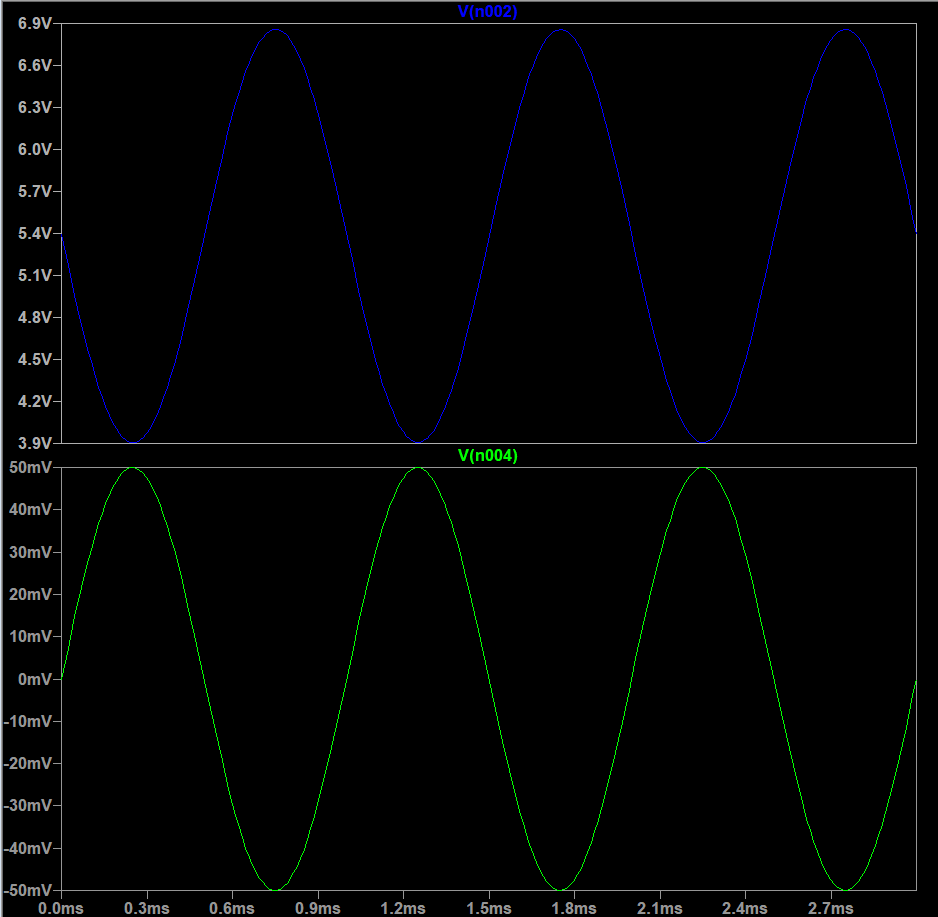
\includegraphics[scale=0.6]{circuit 6 - avdiff}\\\\
				Top pane: \(V_{o1}\), bottom pane: \(V_{i1}\)\\
				\(V_{id}\) = \(V_{i1} - V_{i2}\) = 100mV peak to peak\\
				\(V_{od}\) = \(V_{o1}\) = 2.95V peak to peak\\
				\(A_{Vdiff} = 20log(\frac{V_{od}}{V_{id}}) \)= 29.4 dB.\\\\
				\pagebreak
				\item \textbf{Common mode input analysis}\\\\
				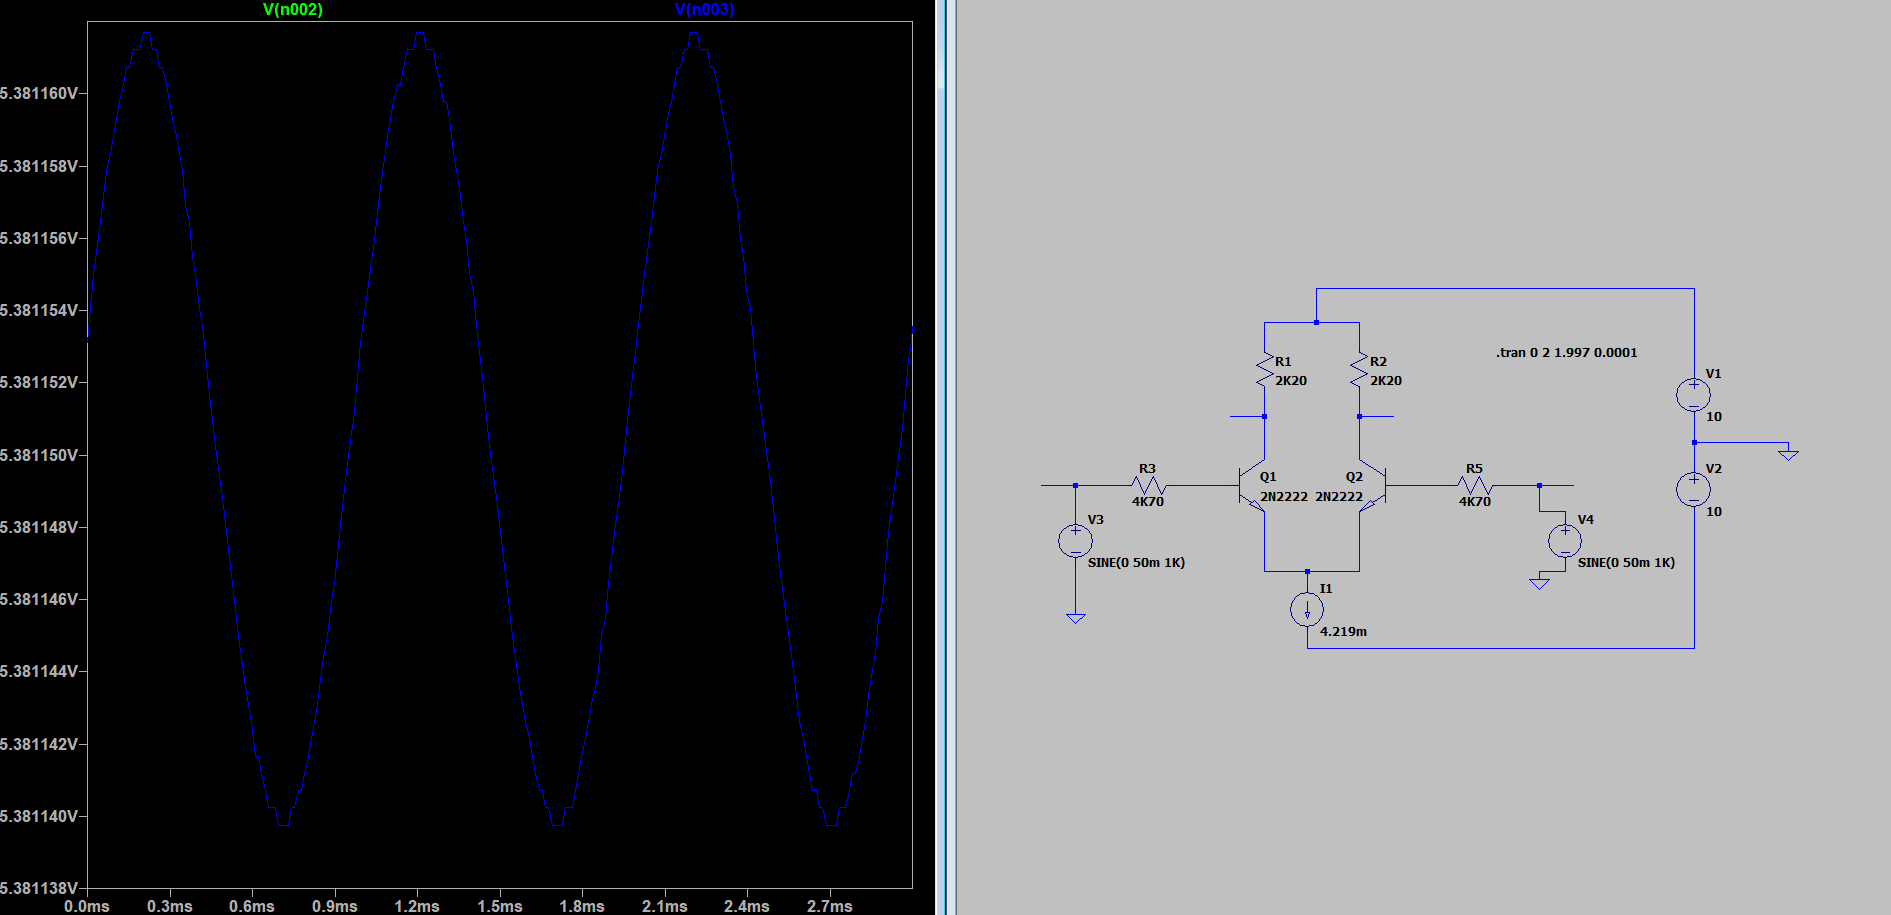
\includegraphics[scale=0.4]{circuit 7 - coll voltages}\\\\
				\(V_C\)(Q1) and \(V_C\)(Q2) are overlapping. (peak to peak: 21.93\(\mu\)V).\\\\
				To calculate \(A_{Vcm}\) I need \(V_{oc}\) and \(V_{ic}\).\\\\
				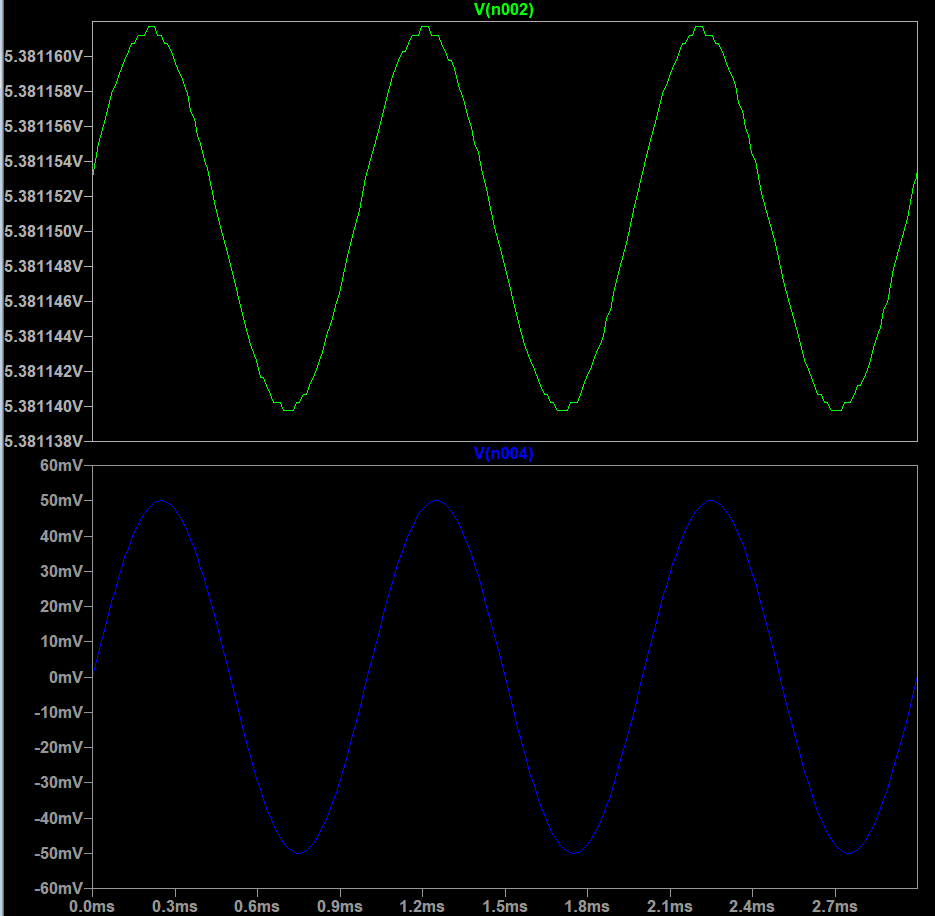
\includegraphics[scale=0.6]{circuit 7 - avcm}\\\\
				Top pane: \(V_{o1}\), bottom pane: \(V_{i1}\)\\\\
				\(V_{ic}\) = \((V_{i1} + V_{i2})/2\) = 100mV peak to peak\\
				\(V_{oc}\) = \(V_{o1}\) = 21.93\(\mu\)V peak to peak\\
				\(A_{Vcm} = 20log(\frac{V_{oc}}{V_{ic}}) \)= -73.28 dB.\\\\
				\item \textbf{Common mode rejection}\\\\
				\(CMRR = 20 log (\frac{A_{Vdiff}}{A_Vcm}) \)= 102.6dB.\\
			\end{enumerate}
		\end{enumerate}
		 
		
	
	
	
\end{document}